\section[How can control engineers help agriculture]{Sidebar: Key cntrol problems in agriculture}\label{sb:ag}


Shortage of qualified human labor is a key challenge facing farmers \cite{richards2018immigration,hertz2013there}, leading to smaller profit margins, and preventing the adoption of truly sustainable agricultural practices. Lack of timely available labor was a principle reason behind the tens of millions of dollars of unharvested fruits and vegetables that rotted in California farms in 2017 \cite{guthman2017paradoxes,RN4026}.  Labor shortage can be a major barrier toome sustainable agricultural practices that are more labor intensive.

Many US agricultural systems (particularly in the Midwest) are dominated by annual row crops such as corn and soybeans. In face of labor shortage, this type of agriculture is practical only with heavy reliance on fertilizers, pesticides, and herbicides, applied over large areas with large equipment. Indeed, in row-crops such as corn and soybean, large industrial scale agriculture is a success story in the United States. In Iowa, for every dollar spent on labor, corn farmers receive \$15-\$20 in income \cite{plastina2018estimated}.  This highly efficient labor to income ratio is primarily because the engineering of large agricultural machines that make it practical to seed, spray, and harvest large fields quickly. For example, a 80' tractor can cover 40 acres an hour driving 6 miles per hour. In combination with highly effective seeds, fertilizers, pesticides, and herbicides, large machines have made large scale monocultures for row-crops like corn, soybean, wheat, barley, and sorghum practical and profitable. However, for these crops, lack of timely and actionable information can lead to potentially excessive use of chemicals and energy despite their potential large negative environmental impact \cite{capellesso2016economic,foley2011solutions,Godfray2010Food}. Indeed, excessive use of herbicides coupled with planting of resistant cultivars is a primary reason behind the proliferation of herbicide resistant weeds in corn and soybean crops in the Midwest \cite{heap2016web,livingston2016economic,gianessi2007value} , while excessive use of nitrogen, herbicides, and insecticides is linked with the potential harm of chemical runoff into US waterways.

More sustainable alternatives that wouldn't need large amounts of chemicals and other inputs, such as perennial polycultures (mixed species of fruit- and nut-producing trees and shrubs \cite{lovell2017temperate}, see Figure \ref{fig:polycultures}), are currently impractical at scale and labor shortage has become a primary barrier to adoption of this sustainable agricultural alternative \cite{RN4017,RN4018}. Polyculture systems can leverage co-habitation of mutually beneficial plants (and  animals) to create a more sustainable engineered ecosystem. % Due to the large variety of complex management tasks required % throughout the growing season 
%to manage polycultures, labor shortage has become a primary barrier to adoption of this sustainable agricultural alternative \cite{RN4017,RN4018}. Indeed, 
%Polycultures are characterized by a level of spatial and temporal variability far greater than prevalent monocultures. 


One way to address the challenges of labor shortage in agriculture is by enabling a tightly integrated chain of information driven technologies that automate the entire production ​chain in agriculture, from seed breeding and chemical production, to farming, and trade of agricultural products. Such an integrated ​digital\textit{ farm of the future} can be enabled if ​data from multiple modalities and platforms is integrated together​ to inform \textbf{​decisions} which can then be transformed into management \textbf{​actions} on the farm with automated equipment. Indeed, there are many ongoing independent efforts to enable the farm of the future: Large equipment companies are automating their equipment and enabling new levels of precision; startups are accelerating the proliferation of small equipment such as drones and small robots for monitoring and management on farms, and data integration and interpretation companies are changing the way growers process, consume, and interact with data.

Here we outline some of the fundamental challenges in autonomy, estimation, and control that the controls community can help overcome to enable the digital farms of the future:

\textbf{Persistent multi-agent autonomy under partial observability}:  The digital farm of the future will employ teams of distributed heterogeneous agents to autonomously manage, optimize, and harvest large acres of diverse crops across the entire season without encumbering humans. This level of autonomy in unstructured field environments is out of reach of the current state-of-the-art which requires constant human monitoring and oversight, especially in the presence of change or unforeseen events. Efficient and reliable control will be central to the success of these robots. Small below-canopy robots (e.g. Figure \ref{fig:terrasentia} \cite{kayacan2018embedded}) will need to provide precision care including pruning, weeding, and re-seeding without damaging plants or causing soil compaction. Deployed at scale, these robots can not only make large scale organic farming practical, but also enable enhanced breeding through  field-scale phenotyping \cite{kayacan2018embedded,mueller2017robotanist,virlet2017field}. \textit{The big controls challenge here is in making decisions over large spatiotemporal scales with information obtained from a few stationary and mobile sensors which can only partially observe the environment at any given time}. The strong theoretical underpinnings in the controls community on autonomy, distributed and networked systems, and estimation can be of tremendous value in engineering digital farm systems consisting of distributed  teams of autonomous agricultural robots.  %The work presented in this paper begins to address this challenge.

\begin{figure}
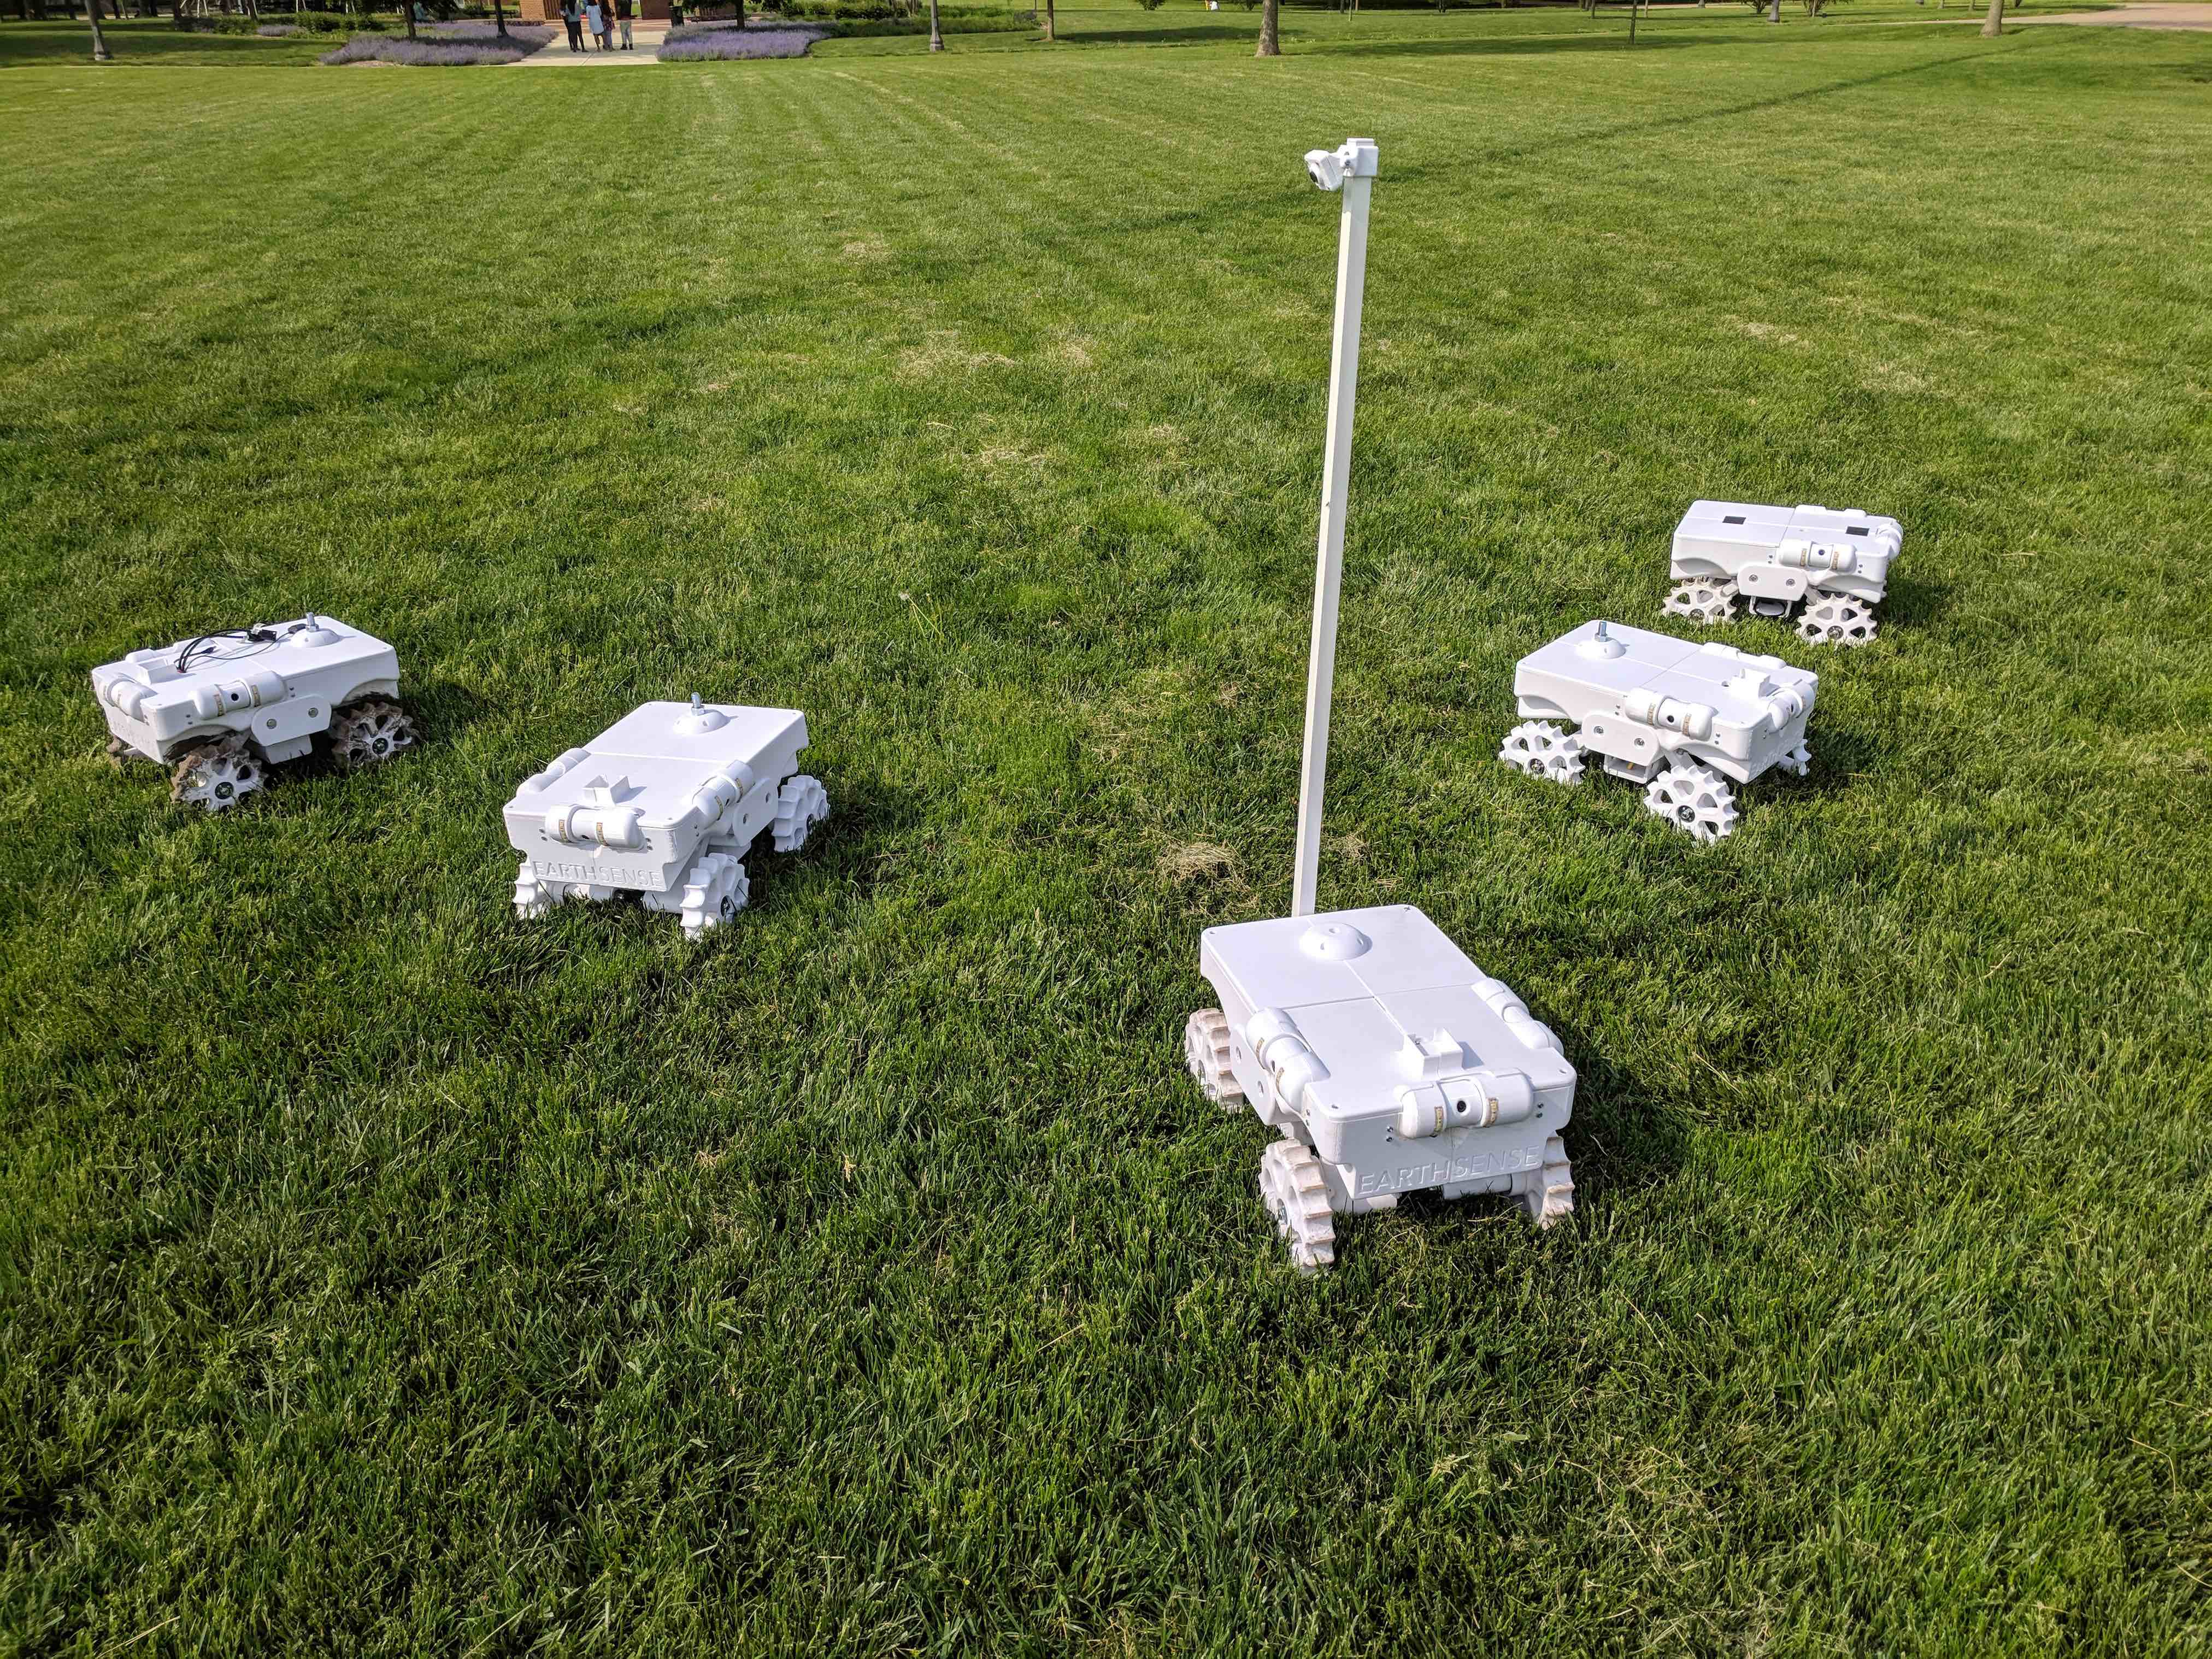
\includegraphics[width=\textwidth]{swarm_robots}
\caption{The TerraSentia robots developed by Chowdhary's group at UIUC and commercialized by EarthSense inc. present exciting possibilities for distributed agricultural management with teams of compact, ultra-light, under-canopy robots equipped with advanced autonomy and machine learning. To make such agricultural robotic systems practical, advances in persistent multi-agent autonomy in field environments are necessary.}
\label{fig:terrasentia}
\end{figure}


%\textbf{Soft robots}

\textbf{Dexterous and ubiquitous robotics for precise care}​: The digital farm of the future will strive to eliminate costly inputs (chemicals, labor, energy, and knowledge) with low-cost, dexterous, and highly autonomous agricultural equipment \cite{pedersen2006agricultural}. Advances in \textit{soft} arms and grippers can enable robots that can have far better reach and dexterity around plants than robots equipped with traditional \textit{hard} industrial robotic arms. Soft arms, which are often actuated with pressurized tubes, can be far less expensive to manufacture and significantly lighter than their hard counterparts. On the other hand, soft arms can be slow to actuate and have limited payloads. To make soft robots practical, optimal feedback control techniques are necessary that work with conformal objects with very large degrees of freedom. In particular, soft arms tend to significantly deform under weight and behave quite differently when loaded with different payloads. Unlike hard arms, encoders are not sufficient to estimate the pose of the arm or the manipulator. Strain and angle sensors need to be positioned judicially to keep costs down, and image based feedback control is often  necessary.  % measurement combined with genome editing and enhanced breeding can help produce seed that perform optimally in specific environments. %and it is difficult to sensing techniques for soft robots that %Significantly early disease detection and treatment can be enabled by teams of over-the-canopy (aerial) and under-the-canopy robots through persistent monitoring in large-scale fields. Advances in machine vision, machine learning, and in-situ sensor data analytics with noisy and spatiotemporally correlated data can drive cost-effective adoption of these technologies. Robotic field-scale phenotype measurement combined with genome editing and enhanced breeding can help produce seed that perform optimally in specific environments. Robotic planting will ensure optimal genotypes are planted in optimal locations across fields.

\textbf{Control of complex designed ecosystems:}   Agricultural ecosystems designed with synergistic biodiversity -- known as \textit{polycultures} -- have long been proposed as alternatives to traditional monoculture-based agriculture \cite{dewar2007perennial,lin2011resilience,thrupp2000linking,letourneau2011does}. Based on studies of a range of natural ecosystems, polycultures are expected to be sustainable, productive, resilient and ecologically beneficial, requiring far less chemical inputs for food production. However, compared to their widely practiced counterparts (traditional monocultures such as corn and soybean), polyculture production systems have not yet been demonstrated to be profitable at large scale. This is primarily %because of two reasons: 1) The lack of dexterous robotic equipment that can be used to perform management tasks in polycultures, and 2) 
%However, polycultures on a large scale have so far been limited 
due to their labor- and knowledge-intensiveness, stemming from their inherent complexity. Indeed, despite their clear benefits and the potential to be profitable, optimizing and managing such complex systems remains a hard problem even for those with training and experience in polycultures. 

%Agriculture inspired by ecosystem principles has been proposed by many \cite{Koohafkan2012a,Molnar2013a} and is practiced on small scales, 

The complex interaction between closely spaced diverse plant species in a polyculture results in both spatial and temporal dynamics as the plants grow and interact with each other. %in polyculture parameters, such as growth rate, plant phenology, and yield. 
Plant growth often exhibits hybrid dynamical systems behavior with rapid thresholded growth bursts followed by slow progression. The triggers for growth bursts are dependent on  environmental factors such as temperature, soil moisture, and sunlight reaching individual and cumulative thresholds, and complex interrelations between neighboring plants, soil chemistry, insects, and soil microbes. 
%Plant growth may best be described by a stochastic hybrid dynamical system with spatial and temporal correlations: Seedling emergence is a discrete probabilistic process that is triggered by environmental factors such as temperature, soil moisture, and sunlight reaching individual and cumulative thresholds. The emergence is also predicated on underlying soil chemistry to be conducive to germination. While temperature, moisture, and sunlight changes at a very rapid temporal scale and broad spatial scales, soil chemistry varies on finer spatial and slow temporal scales. After emergence, seedling growth is characterized by multiple thresholded growth stages, dependent again on the same parameters, however, the progression is more continuous with almost discrete and rapid phase transitions. For example, many plants follow a sigmoidal growth pattern with very slow above ground growth in 5-8 days after emergence, followed by a 3-4 day explosive growth phase, while new seedlings are simultaneously emerging. As a result, the total polyculture population density, growth stages and vigor, can be described by a set of coupled stochastic partial differential equation (PDEs) that with hybrid discrete-continuous dynamics triggered by external factors. %Such hybrid dynamical PDEs are often encountered in many distributed CPS.
Simulating individual plant growth is an active area of research with many open questions in modeling and plant biology \cite{zhu2016plants}. Arguably, very high resolution plant growth models may not even be necessary for effective control of polycultures. Yet on the other hand, the  %TThere are many open problems in modeling 
 %Furthermore, plant growth follows sigmoidal phase transitions: even though  However, 
 existing models of plants and interactions with ecosystems \cite{Stehfest2007a,Foley1996a, Kucharik2003a,Friedl2010a, Rodrigues2010a, Nunes2013a} are not well suited for designing and managing polycultures because of the simplifying assumptions that are often made. A good balance could be struck with data driven machine learning models that have sufficient resolution for aggregate prediction over multiple spatiotemporal scales and are lightweight enough for control and decision making. With these models, predictive control strategies can be created that task teams of robots for management tasks. Furthermore, these predictive models can enable quantified mechanisms of design and planning of efficient agroecosystems. %could strike a good balance between model resolution and . % provide the required fidelity, however, such models would need to predict dynamics over multiple spatial and temporal scales. 
 %The work in this paper presents one approach towards addressing this  modeling an challenge. 
 Obtaining the required data to train these models and using them to create effective control techniques for managing profitable polycultures remains an exciting direction of future work where the control community can help.
 
 The discussion in this sidebar was informed by many conversations with  crop scientists at UIUC. In particular, 
\textit{the authors wish to thank Prof. Stephen Long and Prof. Carl Bernacchi for insights on the phenotyping bottleneck and simulation of plants (\textit{crops-in-silico}), Prof. Adam Davis on inputs on the herbicide resistant weed crisis, and Prof. Sarah Lovell on sustainable agricultural production systems and perennial polycultures.} 

\begin{figure}[tbh]
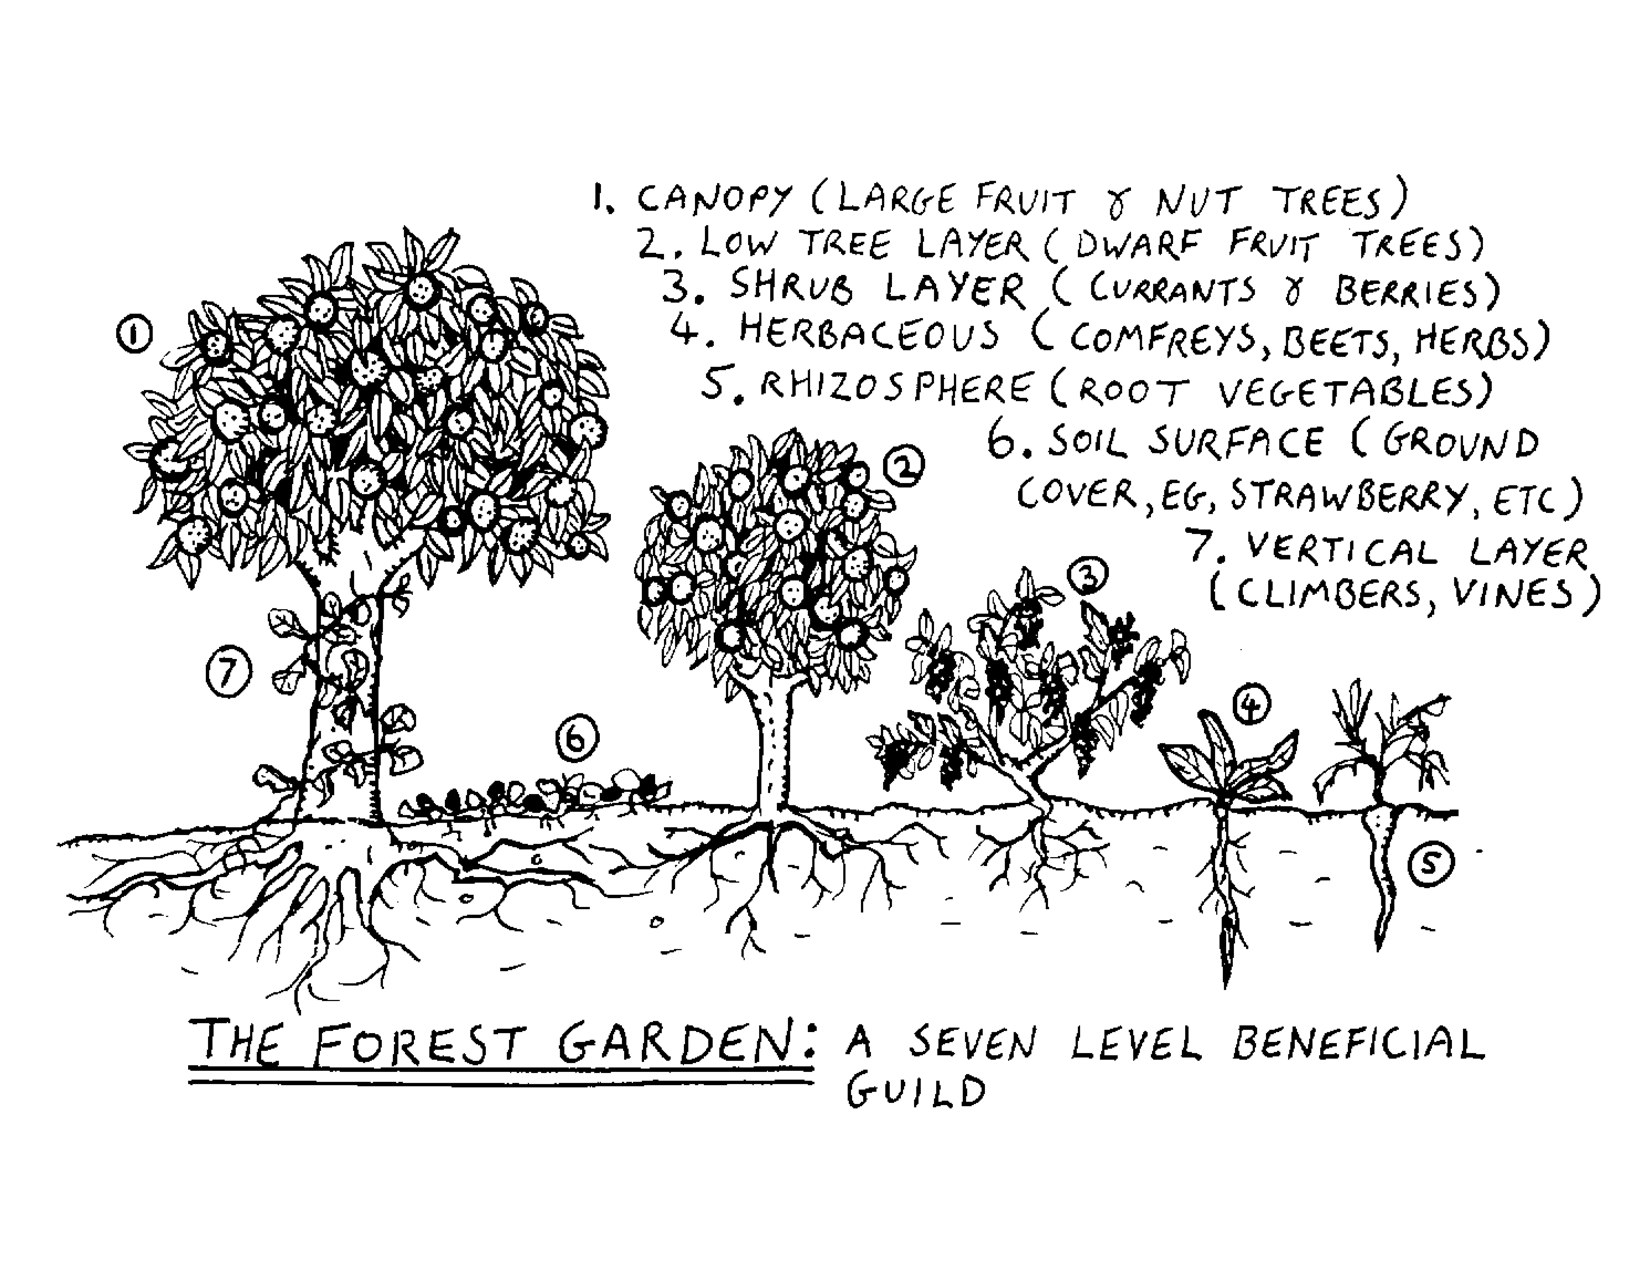
\includegraphics[width=\textwidth]{./figures/polyculture}
\caption{The seven layers of the forest garden. Polyculture agricultural production systems are designed ecosystems that can be more productive and sustainable than traditional monoculture systems. Managing such complex systems requires fundamental advances in robotics, spatiotemporal modeling, and control of complex biological processes, all areas where the control community can help. Figure source \cite{polyculture_fig}  see also \cite{rhodes2012feeding}.}
\label{fig:polycultures}
\end{figure}

%Polycultures are a type of agricultural production system that leverage the interations between different plant species to 

%\textbf{
%Distributed machine learning and predictive modeling driving biology advances}​: New learning and inference algorithms are needed to enable a team of distributed sensors to predict quantities of interests across large farms with only partial observations. Machine learning needs to be able to consume large volumes of unstructured unlabeled data to find hidden patterns that drive advances in plant biology and plant care, and utilize this understanding to improve crop productivity and management techniques.
